\documentclass[12pt]{article}
\usepackage{graphicx}
\usepackage{wrapfig}
\usepackage{subfigure}
\usepackage{multirow}
\usepackage{hyperref}
\usepackage{amsmath}
\usepackage{amssymb}
%\usepackage{ngerman}
\usepackage[ansinew]{inputenc}
\usepackage[left=2cm,top=1cm]{geometry}

% vector graphics test
\usepackage{color}
\usepackage{transparent}
\graphicspath{{graphs/}}

\setlength{\parindent}{0pt}

%\usepackage[outdir=./]{epstopdf}
%\epstopdfsetup{outdir=./}


\begin{document}
	\pagestyle{empty}
	

\begin{titlepage}
	\centering
	\bigskip
	\huge{Astronomisches Praktikum:\\Planetenbahnen}\\
	\bigskip
	\large{Versuch 8}\\
	\bigskip
	\large{Jan R\"{o}der \& Julia Lienert}
	\bigskip
	\tableofcontents
\end{titlepage}

\pagebreak


\section{Einleitung}

\section{Grundlagen}

\subsection{Aufgabe 1}

\paragraph{Erstes Gesetz.} Stellt man die Energiegleichung bzw. das Gravitationsgesetz f�r einen K�rper mit Masse $m$ um eine zentrale Masse $M$ auf, erh�lt man nach Umformung einen Kegelschnitt:
\begin{equation}
r(\phi) = \frac{P}{1+e\cdot cos(\phi)}
\end{equation} 
mit dem Halbparameter $P$ und der Elliptizit�t $e$. Es sind somit drei Arten von Umlaufbahnen m\"{o}glich:
\begin{align*}
e < 1  &: \ \ \text{Ellipse}   \\
e = 1  &: \ \ \text{Parabel}   \\
e > 1  &: \ \ \text{Hyperbel}  
\end{align*}
F\"{u}r die Planetenbahnen gilt $e<1$, sie sind Ellipsenbahnen. In einem der Brennpunkte dieser Ellipsen steht jeweils die Sonne (f\"{u}r jeden Planeten).
\paragraph{Zweites Gesetz.} Zieht man von der Sonne zu einem der Planeten einen ``Fahrstrahl'' und l�sst den Planeten loslaufen, stoppt man die Zeit zu Beginn der Bewegung. Nach einem bestimmten Zeitintervall wurde vom Fahrstrahl eine Fl�che aufgespannt, die direkt zur gestoppten Zeit geh�rt. Das bedeutet: in gleichen Zeitabschnitten werden gleiche Fl�chen �berstrichen.
\paragraph{Drittes Gesetz.} Die Umlaufzeit $T$ im Quadrat und die dritte Potenz der gro�en Halbachse $a$ stehen also f�r eine Planetenbahn in einem bestimmten, konstanten Verh\"{a}ltnis. 
\begin{equation}
\frac{T^2}{a^3} = const. = \frac{4\pi ^2}{G(M+m)}
\end{equation}
Dabei wird die Annahme getroffen, dass die Planetenmasse $m$ gegen�ber der Sternmasse $M$ gering ist.

\subsection{Aufgabe 2}

Die Ekliptik ist definiert als diejenige Ebene, in der sich die Sonne in einem Jahr vor dem Fixsternhimmel scheinbar �ber den Himmel bewegt. \\
Eine Planetenbahn wird charakterisiert durch die folgenden Grundgr��en: Inklination (Orientierung gegen�ber dem �quator des Koordinatensystems), Exzentrizit�t bzw. die Halbachsen (Form der Umlaufbahn) und die L�nge des aufsteigenden Knotens (Schnittpunkt mit dem �quator des Systems).

\subsection{Aufgabe 3}

W�hlt man ein astronomisches Koordinatensystem zur verwendung, wird es Objekte geben, die sich relativ dazu bewegen. Dies wird als Positionsdaten mit Zetiverlauf festgehalten; diese Daten nennt man Ephemeriden. Die Ephemeriden werden in gleichen Zeitintervallen katalogisiert. 

\subsection{Aufgabe 4}

Um die Frage zu kl�ren, warum Pluto nicht mehr als Planet gez�hlt wird, muss man die Definition eines Planeten betrachten:
\begin{enumerate}
	\item Ein Planet bewegt sich immer um einen zentralen Stern, nie um einen anderen Planeten.
	\item Durch hydrostatisches Gleichgewicht und die eigene Gravitation hat das Objekt ann�hernd Kugelform.
	\item Das Objekt ist massereich genug, um seine Umlaufbahn um den Stern von Asteroiden und anderen Kleink�rpern freizur�umen.
\end{enumerate}
Das letzte Kriterium kann Pluto aufgrund seiner geringen Masse und seines gro�en Orbits nicht erf�llen.


\section{Die geozentrische Plutobahn}

\subsection{Aufgabe 4}

Die Eigenbewegung des Pluto erh�lt man mithilfe zweier Punkte, die m�glichst genau ein Jahr auseinander liegen. Hier sind das:
\begin{table} [h]
	\centering
	\begin{tabular}{|c|c|c|}
		\hline
		Datum	& Rektaszension $\alpha$	& Deklination $\delta$			\\ \hline
		29.08.1979	& 13\,h 31\,m 45.0\,s		& $+$8\,� 26\,' 3.7\,"     		\\ \hline
		23.08.1980  & 13\,h 40\,m 1.3\,s		& $+$7\,� 38\,' 42.1\,"			\\ \hline
	\end{tabular}
	\caption{Ben�tigte Sterndaten zur Ermittlung der Eigenbewegung von Pluto}
	\label{tab:Daten}
\end{table}
Damit gilt $\Delta\delta=0.7893\text{\,}\mathring{}$ und $\Delta \alpha = 2.0679\text{\,}\mathring{}$. Letzteres ist die Rektaszensionsdifferenz, wenn man die Umrechnung in Grad durchf�hrt, in dem man alle Werte mit 15\,$\mathring{{}}$ multipliziert. Dies muss nun mit $\cos \bar{\delta}$ korrigiert werden. Man erh�lt $\Delta\alpha=2.0476\text{\,}\mathring{}$. Die beiden Differenzen sind nun die Werte f�r ein Jahr, man muss also durch 12 teilen und die Werte nochmals Umrechnen, um die Eigenbewegung herauszurechnen.


\section{Das Erde-Mond-System}

\subsection{Aufgabe 1}

Die Mondumlaufbahn ist keine einfache Kepler-Bahn um die Erde. Sie wird zus�tzlich beeinflusst durch die gravitativen Einfl�sse anderer Planeten (vor allem Jupiter) sowie der Sonne. Au�erdem ist die Erde keine perfekte Kugel, was kleine St�rungen in der Mondumlaufbah verursacht, da Gravitationskr�fte dann nicht gleichm��ig angreifen.

\subsection{Aufgabe 2}

Aus den Ephemeriden der Sonne �ber ein Jahr kann man Zeit und ekliptikale Breite extrahieren. Gegeneinander aufgetragen erkennt man, dass die ekliptikale Breite um die 0\,$\mathring{}$ - Marke schwankt. Dies liegt an den Kr�ften des Mondes, ohne den die Schwankung noch viele Gr��enordnungen geringer w�re. Durch die periodische Mondbahn ver�dert sich auch die ekliptikale Breite, da sich Erde und Mond um ein gemeinsames Baryzentrum bewegen.

\subsection{Aufgabe 3}




\section{Diskussion}






\section{Quellen}
\begin{enumerate}
	\item Versuchsanleitung zu Versuch 6: "Teleskope und Astrometrie"
	\item https://de.wikipedia.org/wiki/Parallaxe
\end{enumerate}


%\begin{figure} [h]
%	\centering
%	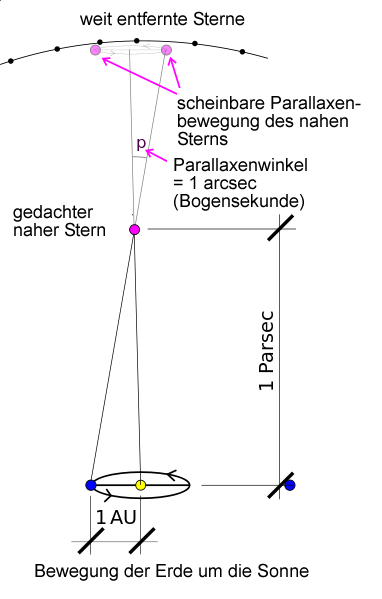
\includegraphics[width=0.4\textwidth]{2_4_Parallaxe.png}
%	\caption{Skizze zur Erkl�rung der Parallaxe (entnommen aus [2])}
%	\label{fig:Parallaxe}
%\end{figure}








\end{document}